\section*{1.B}

	{\Large Zadání:} \\
	$U_1 = 95 \text{V} \; U_2=115 \text{V}$ \\
	$R_1 = 650 \Omega \; R_2 = 730 \Omega \; R_3 = 340 \Omega \;
	R_4 = 330 \Omega \; R_5 = 410 \Omega \; R_6 =830 \Omega$ \\
	$R_7 = 340 \Omega \; R_8 = 220 \Omega$

	$U_{R_8} = \: \text{?}$ \\
	$I_{R_8} = \: \text{?}$ \\

	\begin{figure}[H] 
		\vspace{-1.1cm}
		\center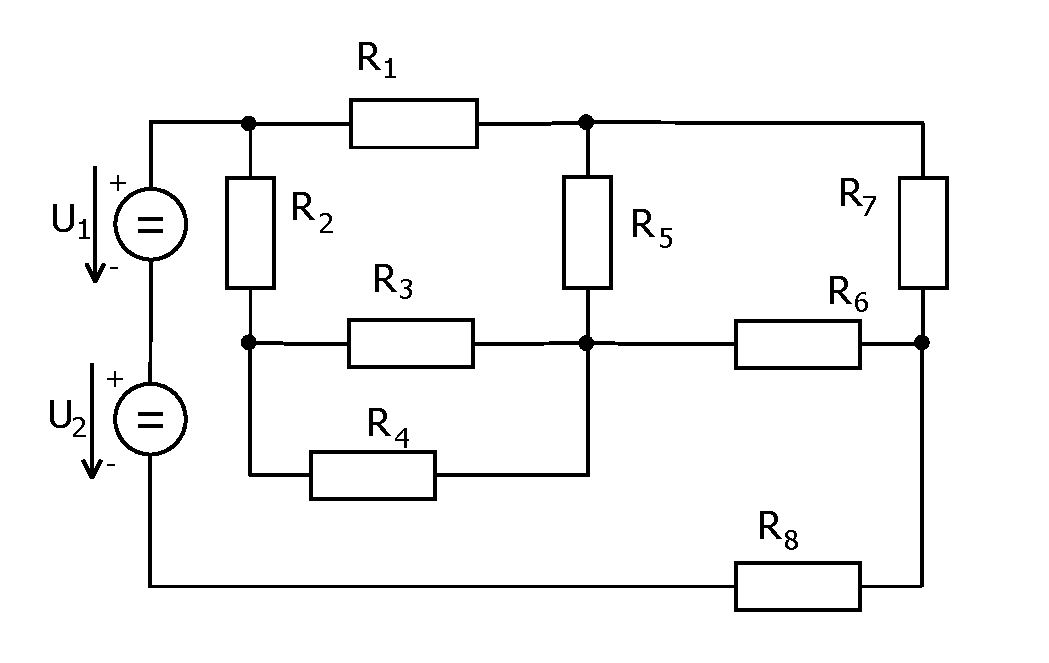
\includegraphics[width=0.6\linewidth]{obr/1_1}
	\end{figure}

	{\Large Řešení metodou postupného zjednodušování}\\

	\begin{figure}[H]
		\center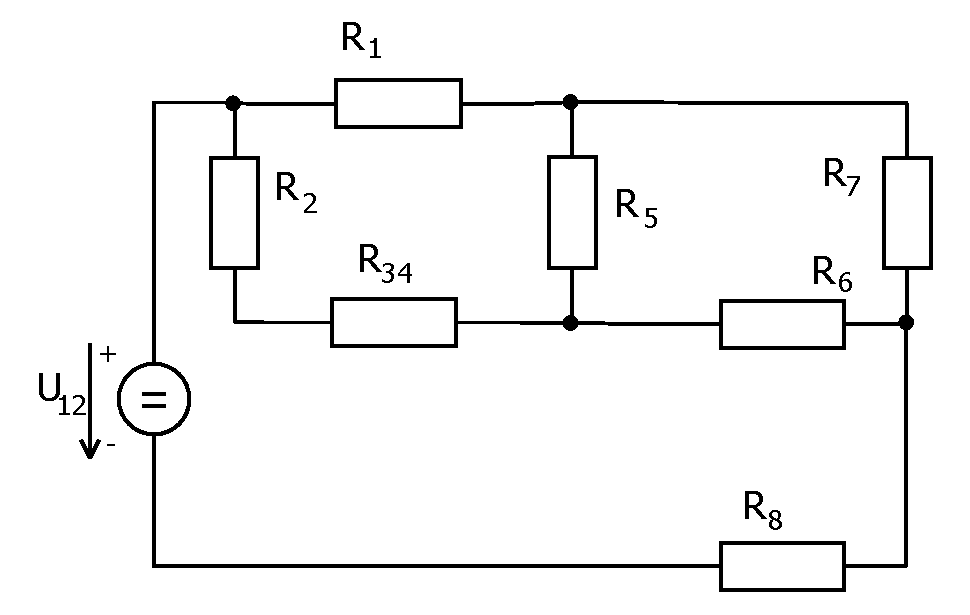
\includegraphics[width=0.6\linewidth]{obr/1_2}
		\caption*{$R_3$ a $R_4$ jsou zapojeny paralelně a zdroje $U_1$ a $U_2$ sériově }
	\end{figure}
	\begin{gather*}
		R_{34} = \frac{R_3 R_4}{R_3 + R_4} =\frac{340 \cdot 330}{340 + 330} \doteq 167.4627 \Omega \\
		U_{12} = {U_1 + U_2} = {95 + 115} = 210  \text{V}
	\end{gather*}

	\begin{figure}[H]
		\center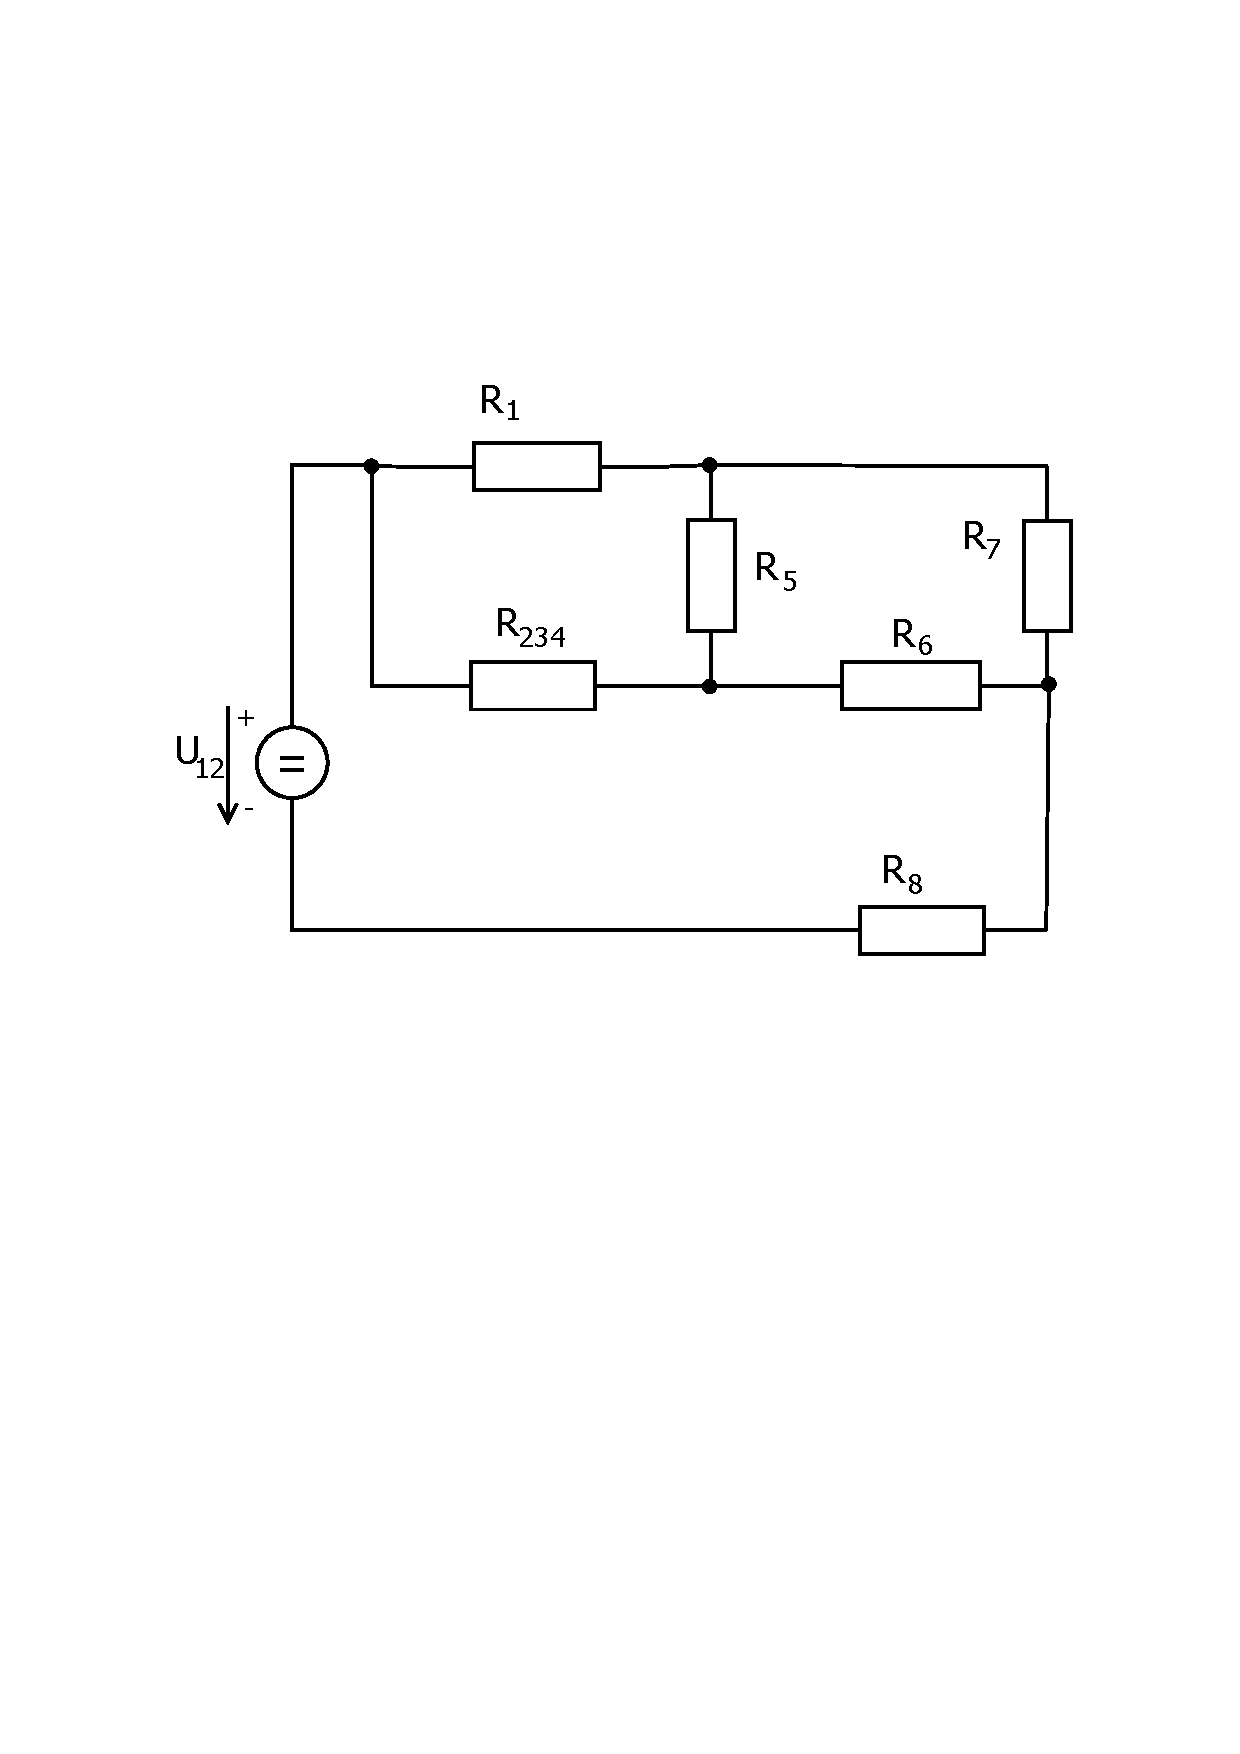
\includegraphics[width=0.6\linewidth]{obr/1_3}
		\caption*{$R_2$ a $R_{34}$ jsou zapojeny sériově}
	\end{figure}
	\begin{gather*}
		R_{234} = R_2 + R_{34} = 730 + 167,4627 = 897,4627 \Omega
	\end{gather*}

	\begin{figure}[H]
		\vspace{-1.1cm}
		\center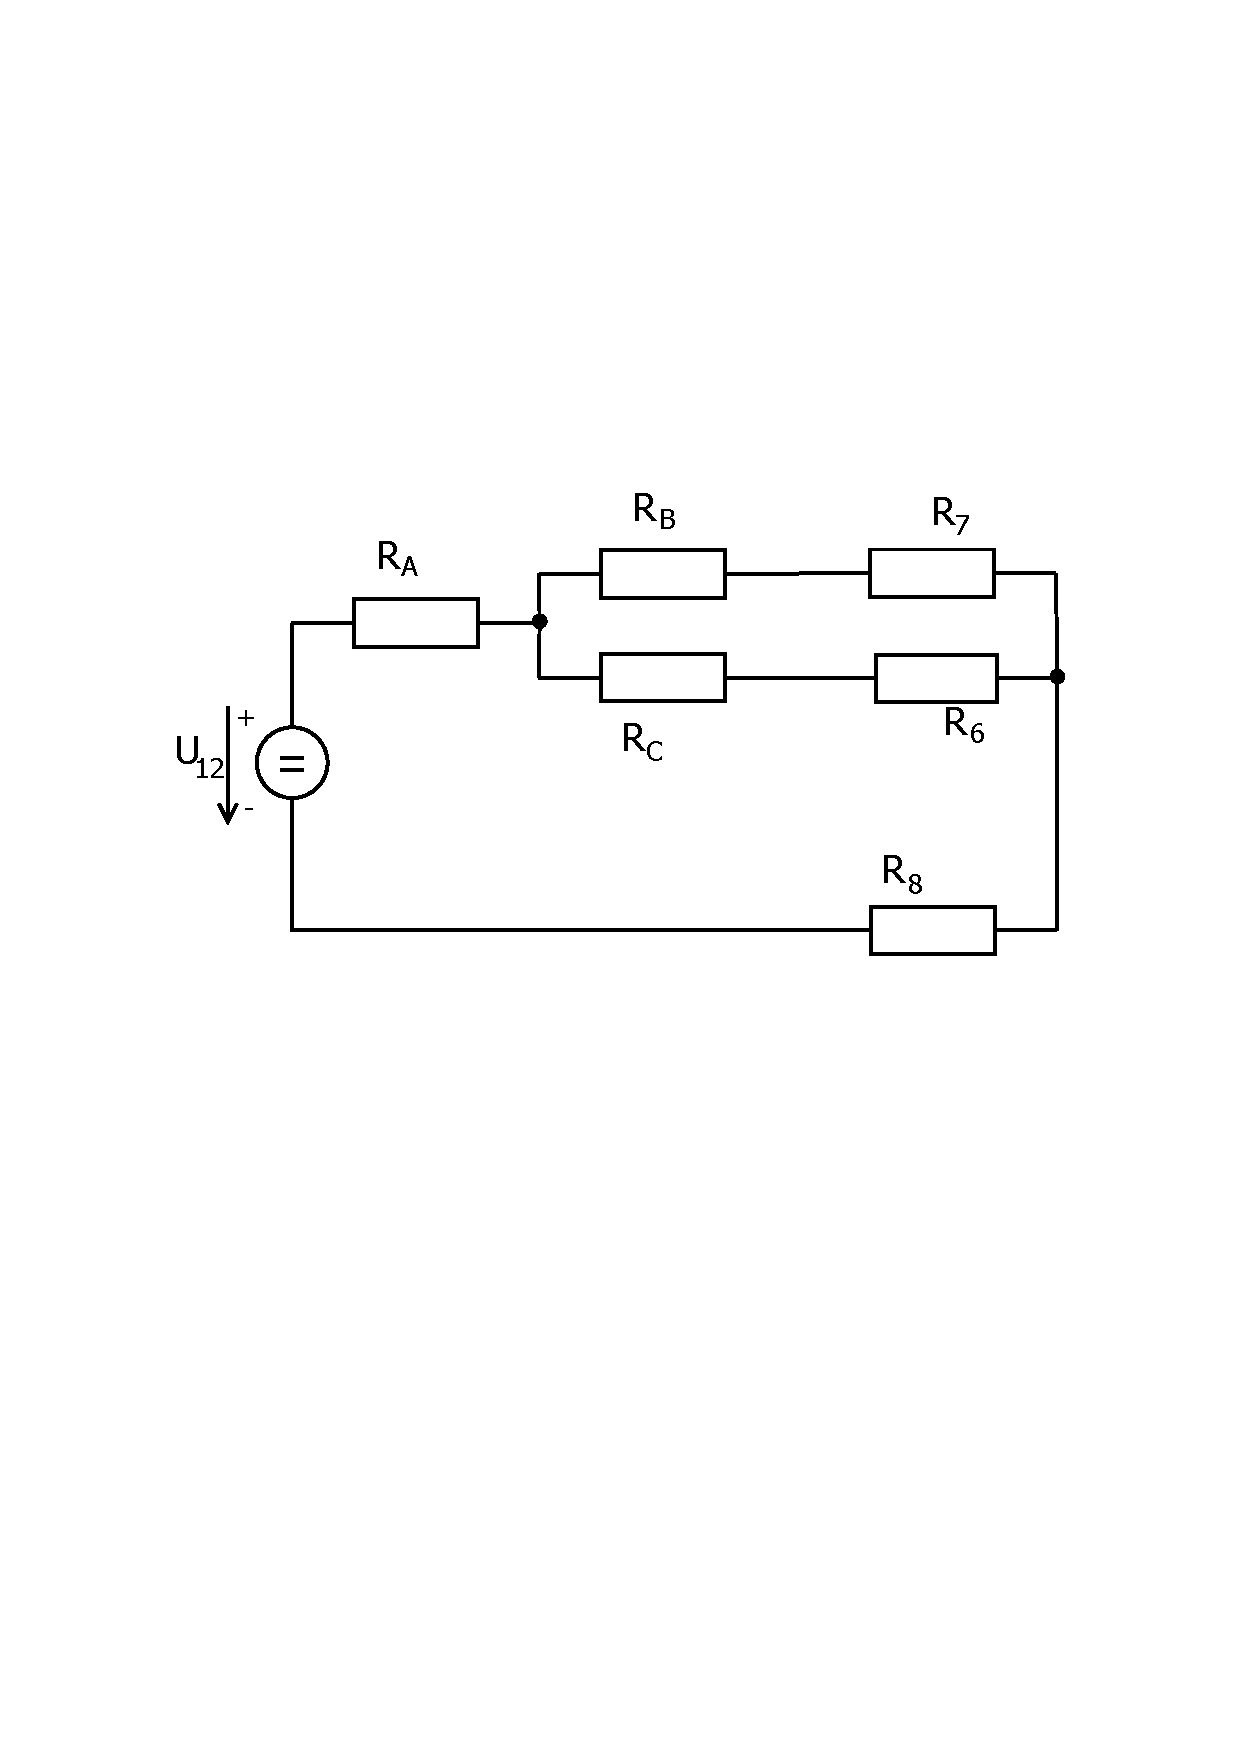
\includegraphics[width=0.6\linewidth]{obr/1_4}
		\caption*{transfigurace - trojúhelník}
	\end{figure}
	\begin{gather*}
		R_A = \frac{R_1  R_{234}}{R_1 + R_{234} + R_5} = \frac{650 \cdot 897,4627}{650 +  897,4627 + 410} = 298,0132 \Omega \\
		R_B = \frac{R_1  R_5}{R_1 + R_{234} + R_5} = \frac{650 \cdot 410}{650 +  897,4627 + 410} = 136,1456 \Omega \\
		R_C = \frac{R_5  R_{234}}{R_1 + R_{234} + R_5} = \frac{410 \cdot 897,4627}{650 +  897,4627 + 410} = 187,9779 \Omega 
	\end{gather*}

	\begin{figure}[H]
		\center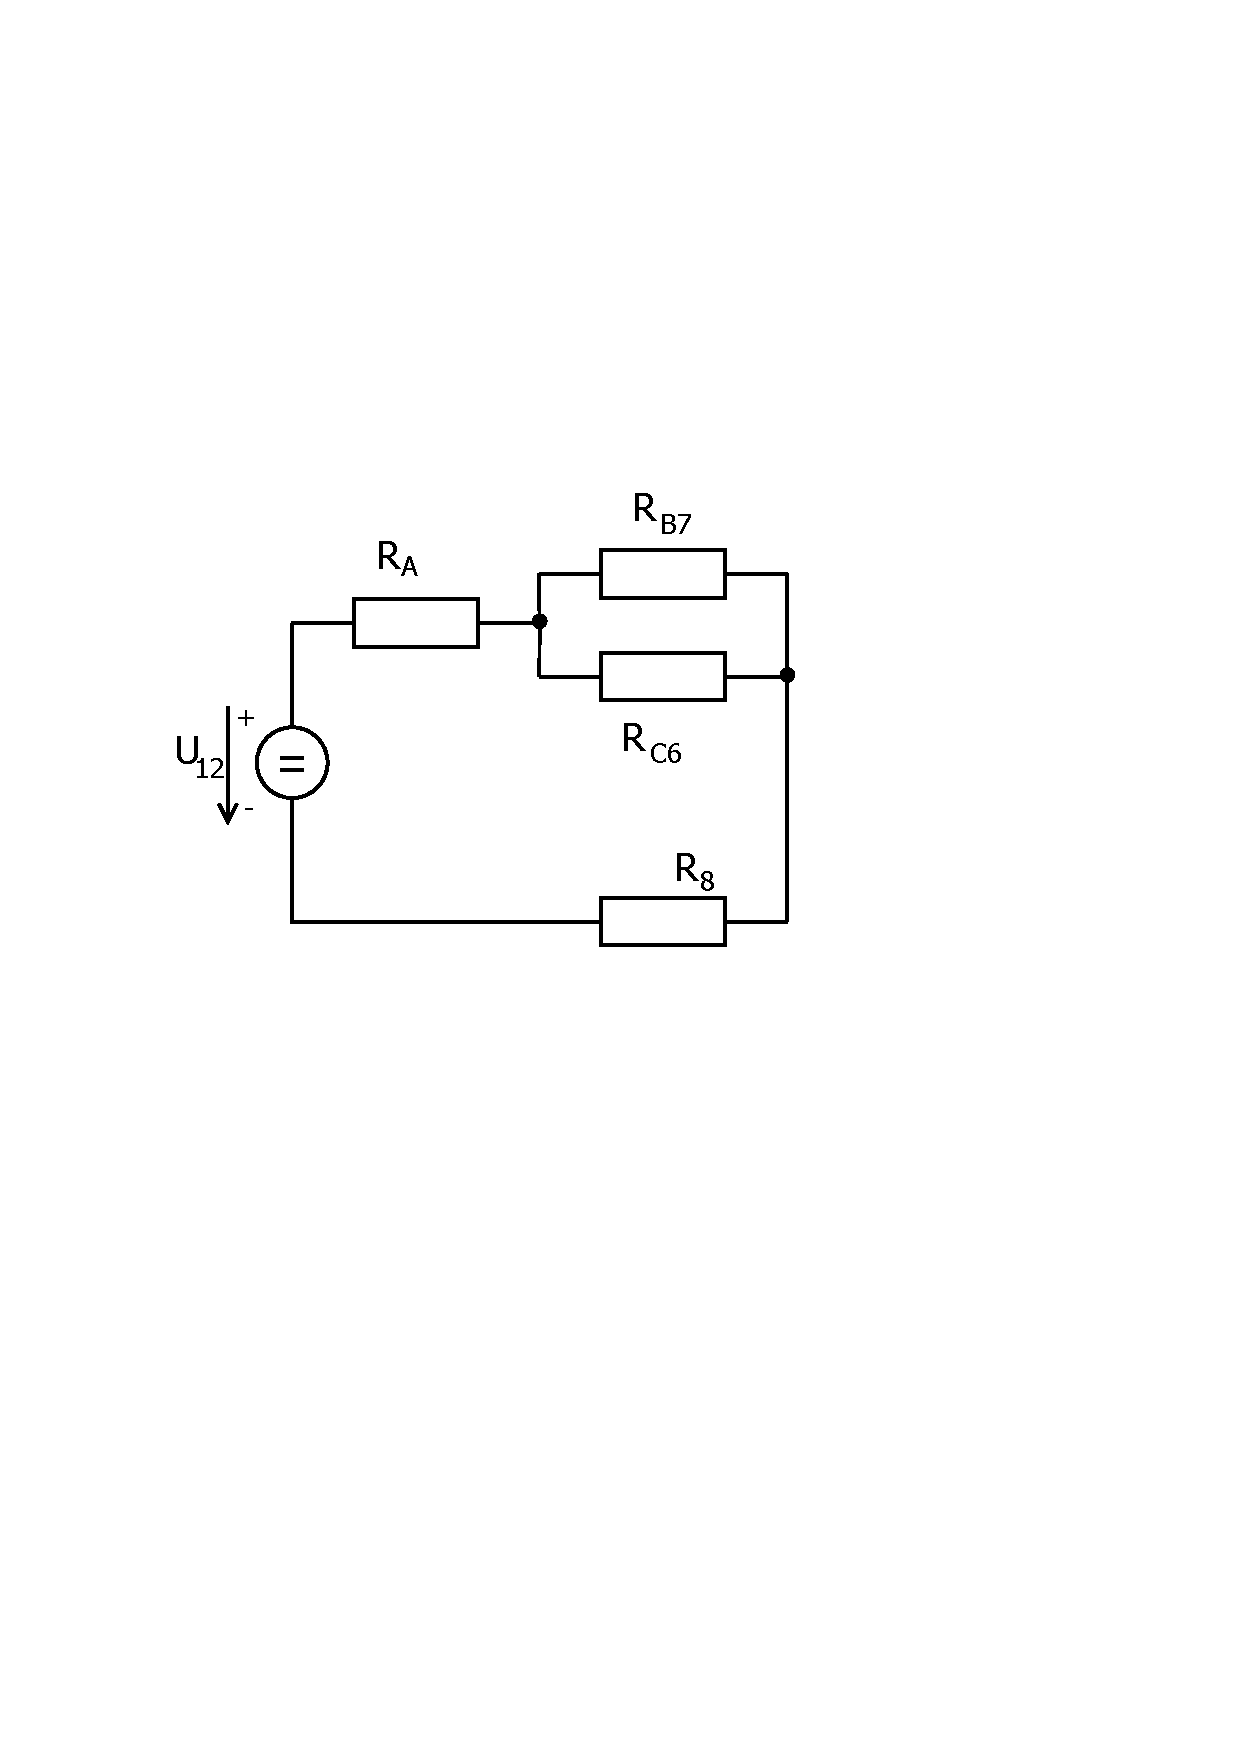
\includegraphics[width=0.6\linewidth]{obr/1_5}
		\caption*{$R_B$ a $R_7$ jsou zapojeny sériově stejně jako $R_C$ a $R_6$}
	\end{figure}
	\begin{gather*}
		R_{B7} = R_B + R_7 = 136,1456 + 340 = 476,1456 \Omega \\
		R_{C6} = R_C + R_6 =187,9779 + 830 = 1017,9779 \Omega
	\end{gather*}


	\begin{figure}[H]
		\center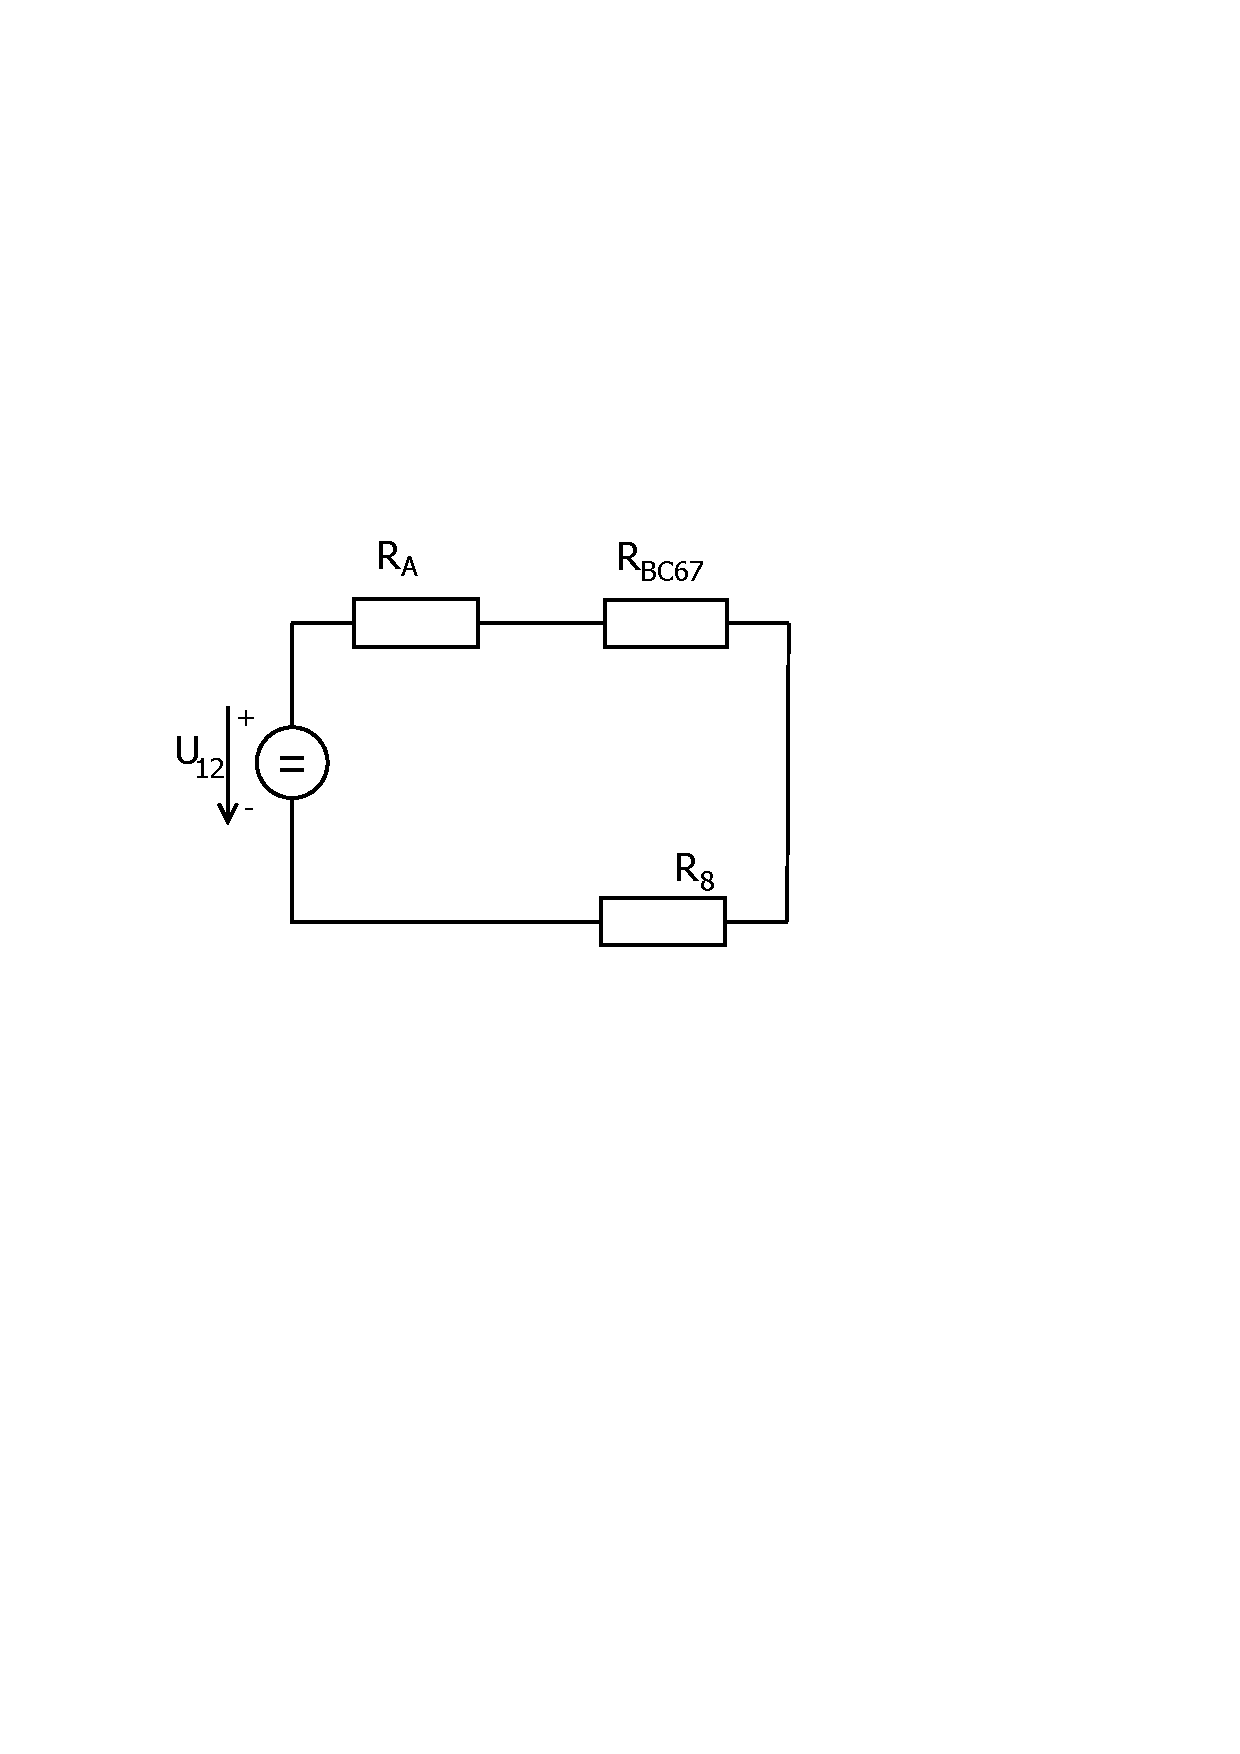
\includegraphics[width=0.6\linewidth]{obr/1_6}
		\caption*{ $R_{B7}$ a $R_{C6}$ jsou zapojeny paralelně}
	\end{figure}
	\begin{gather*}
		R_{BC67} = \frac{R_{B7} R_{C6}}{R_{B7} + R_{C6}} = \frac{476,1456 \cdot 1017,9779}{476,1456 + 1017,9779} = 324,4081 \Omega
	\end{gather*}

	\begin{figure}[H]
		\center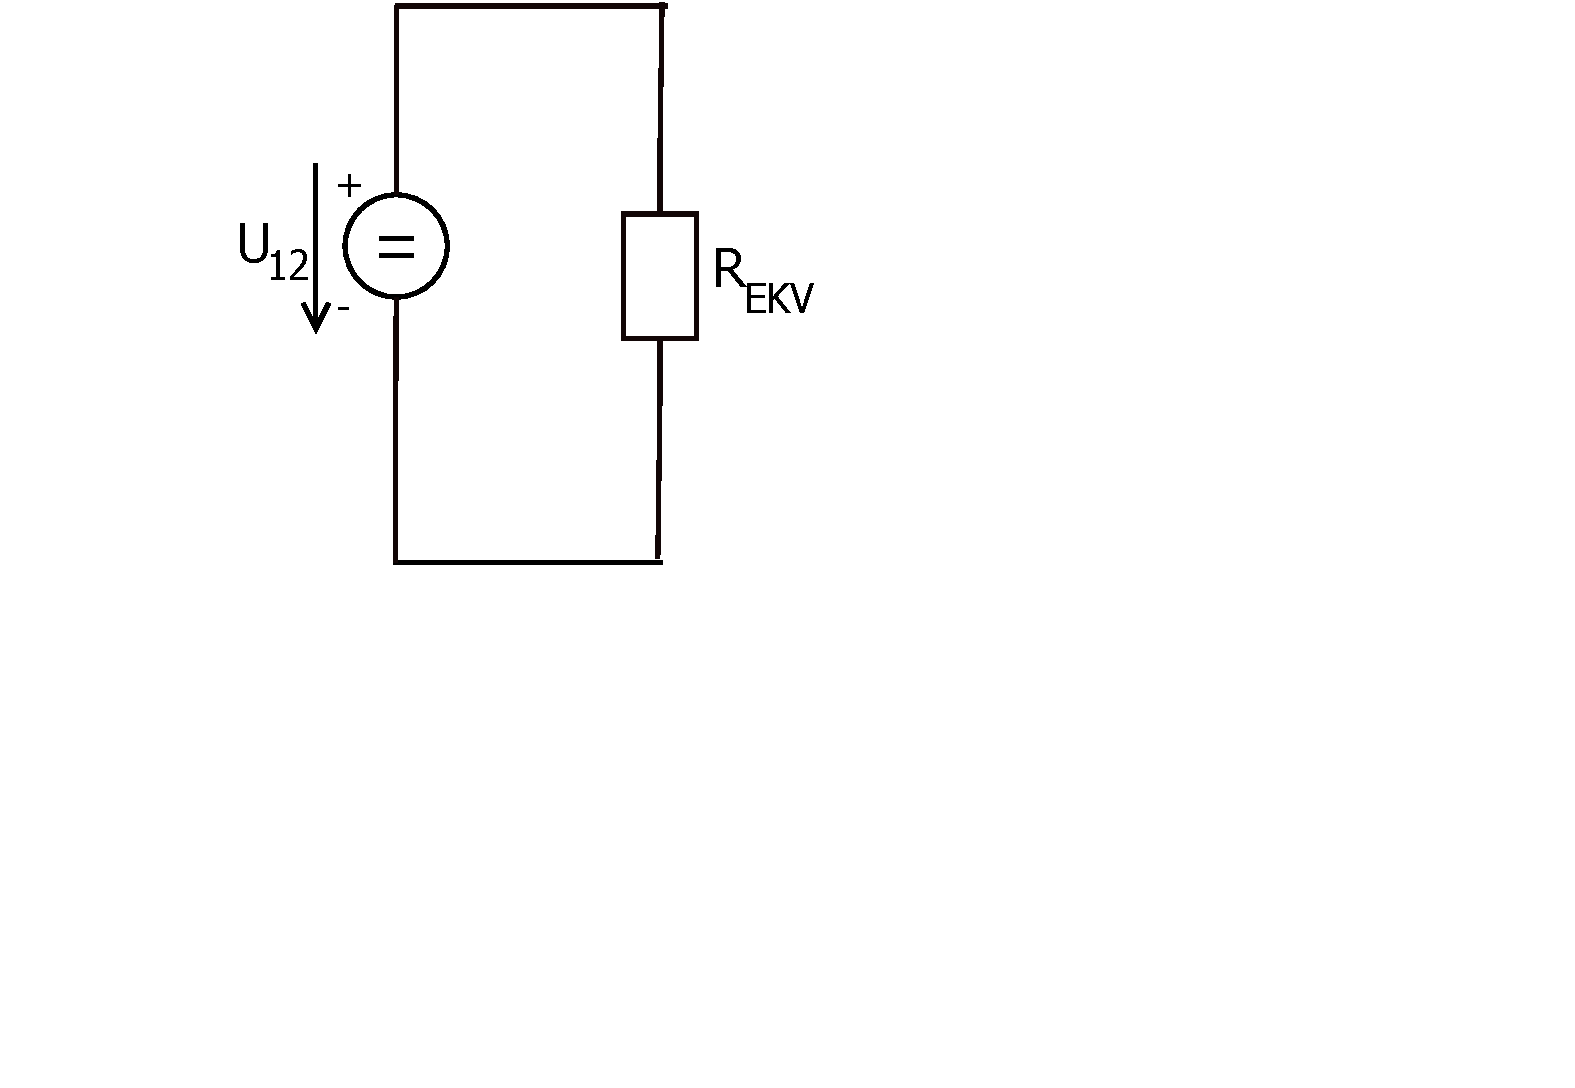
\includegraphics[width=0.3\linewidth]{obr/1_7}
		\caption*{$R_A$ a $R_{BC67}$ a $R_8$ jsou zapojeny sériově - získáváme $R_{EKV}$}
	\end{figure}
	\begin{gather*}
		R_{EKV} = R_{A} + R_{BC67} + R_8 = 298,01232 + 324,4081 + 220 = 842,4213 \Omega
	\end{gather*}

	Celkový proud $I$:
	\begin{gather*}
		I = \frac{U_{12}}{R_{EKV}} = \frac{210}{842,4213} \doteq 0,2493 \text{A}
	\end{gather*}

	Začneme zpětně počítat napětí a proudy, až dojdeme k $U_{R_6}$ a $I_{R_6}$:

	\begin{figure}[H]
		\center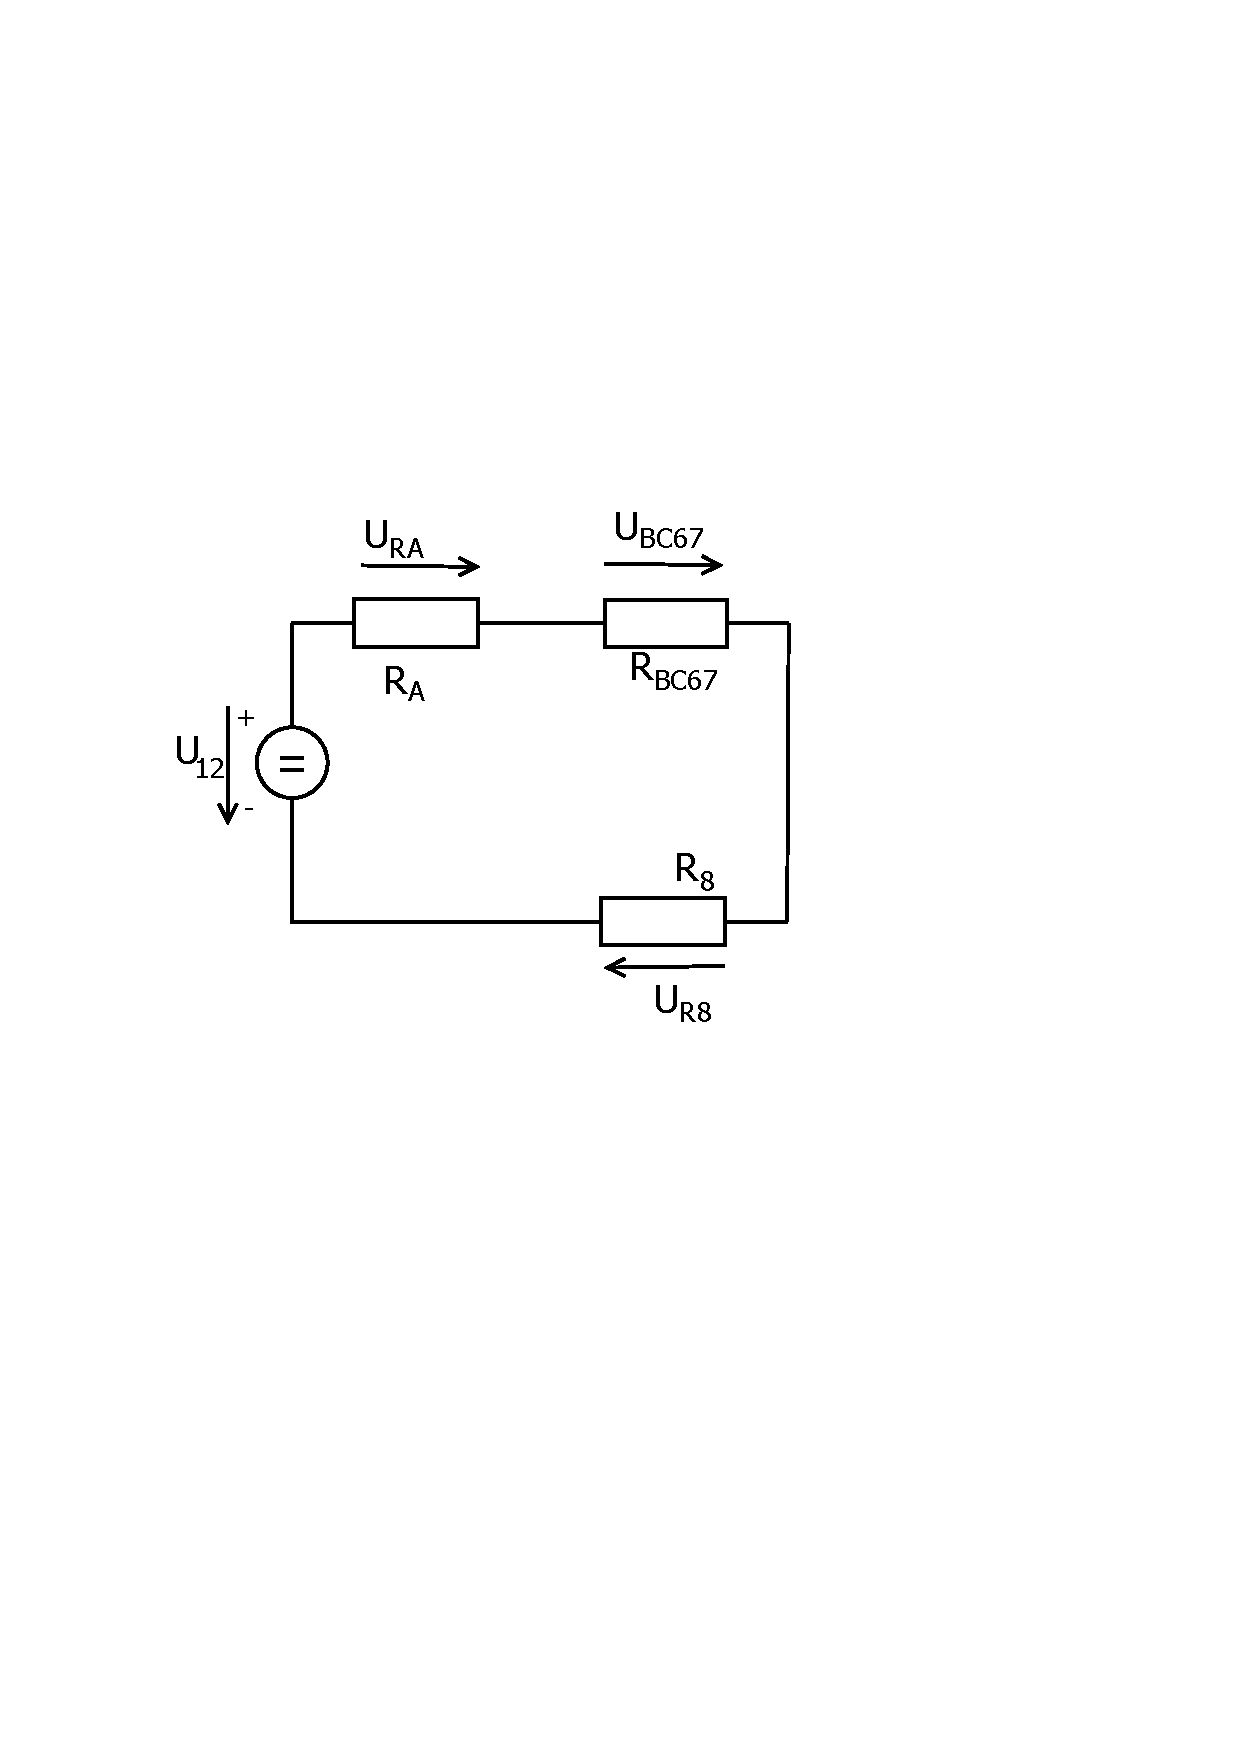
\includegraphics[width=0.6\linewidth]{obr/1_8}
		\caption*{Spočítáme si napětí na jednotlivých odporech}
	\end{figure}
	\begin{gather*}
		U_{R_A} = {I R_A} = {0,2493\cdot 298,0132} \doteq 74,2947  \text{V} \\
		U_{R_{BC67}} = {I R_{BC67}} = {0,2493 \cdot 324,4081} \doteq 80,8749  \text{V} \\
		U_{R_8} = {I R_8} = {0,2493 \cdot 220} = 54,846  \text{V} \\
		\\
		\text{Provedeme kontrolu pomocí II. Kirchhoffova zákona.}  \\
		U_{R_A} + U_{R_{BC67}} + U_{R_8} - U_{12} =  0 \\
	\end{gather*}

	\begin{figure}[H]
		\center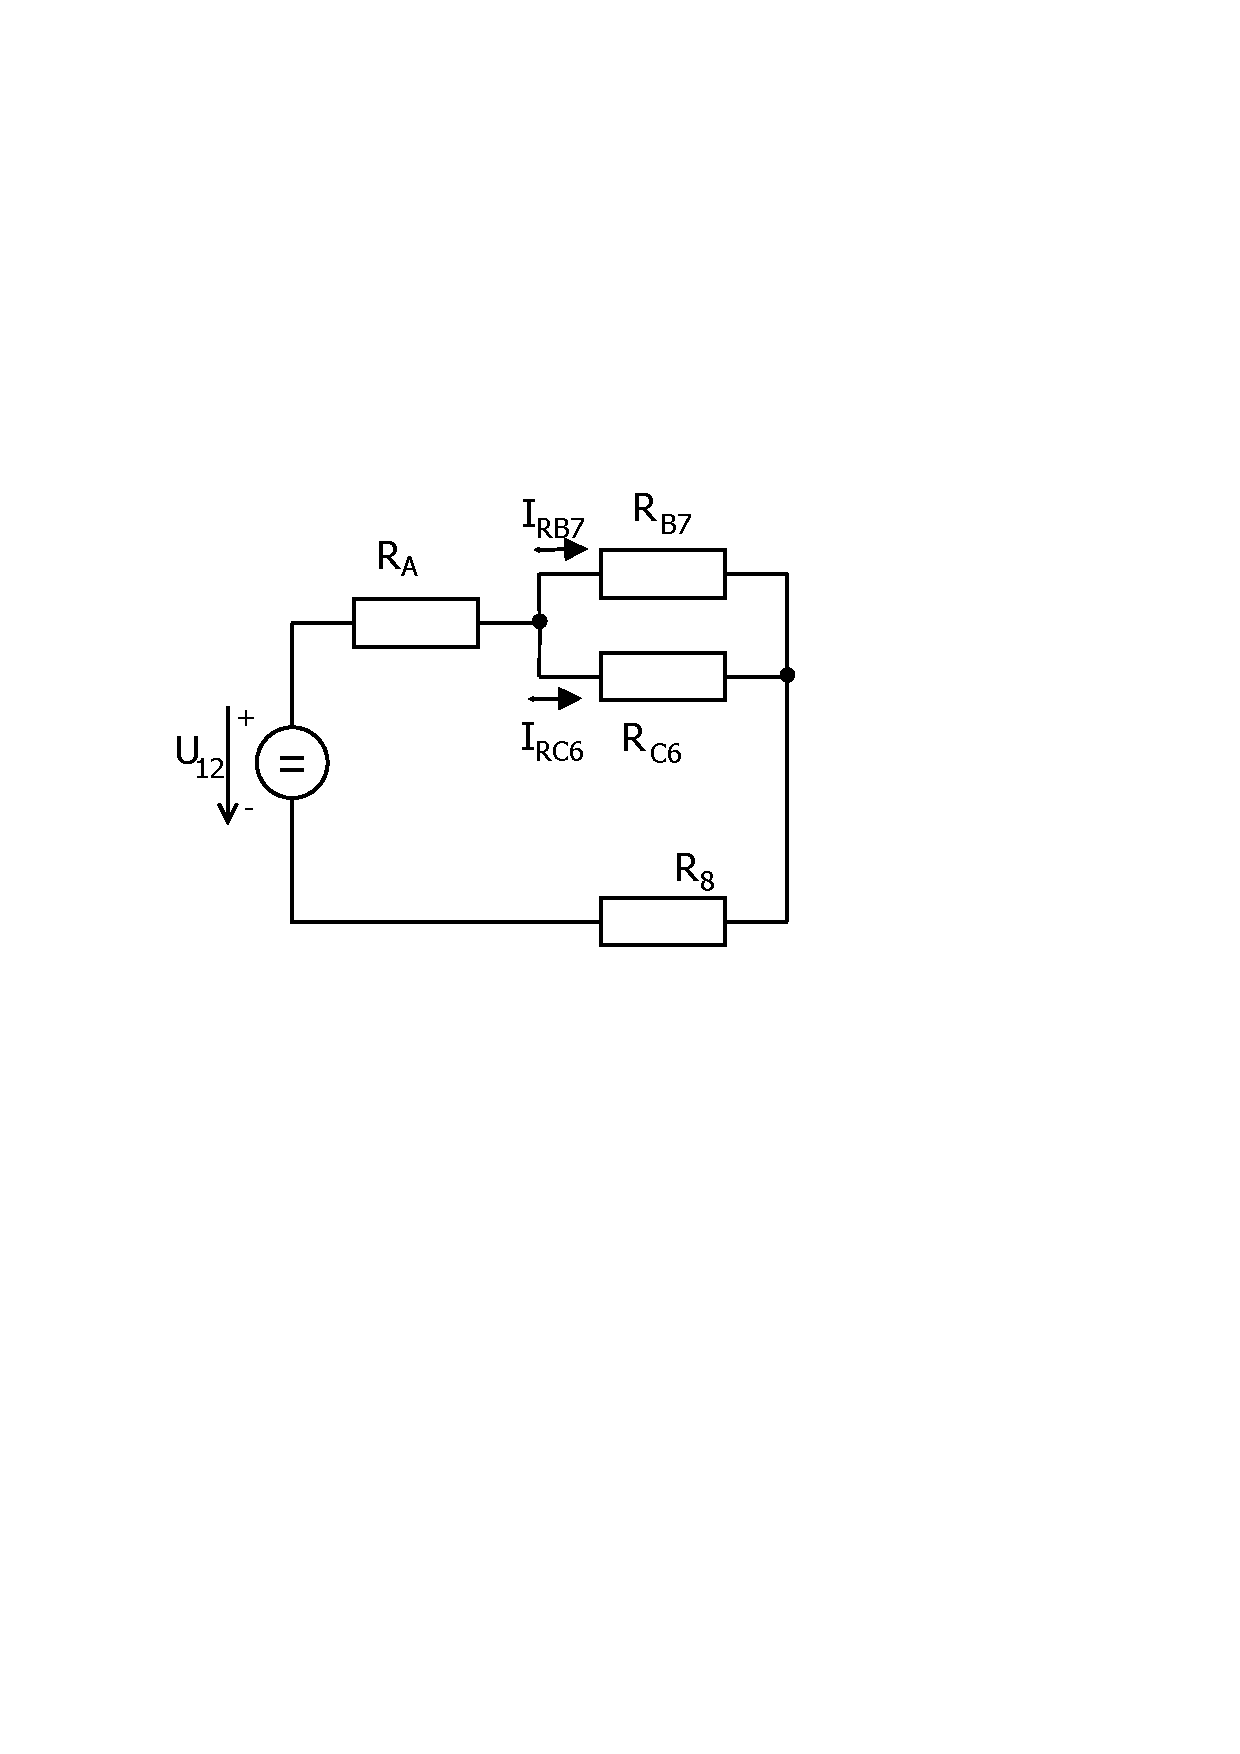
\includegraphics[width=0.6\linewidth]{obr/1_9}
		\caption*{Spočítáme si proud ve větvích s $R_{B7}$ a  $R_{C6}$}
	\end{figure}
	\begin{gather*}
		I_{R_{B7}} = \frac{U_{R_{BC67}}{R_{B7}}} = \frac{80,8749}{476,1456} \doteq 0,1699 \text{A} \\
		I_{R_{C6}} = \frac{U_{R_{BC67}}{R_{C6}}} = \frac{80,8749}{1017,9779} \doteq 0,0794 \text{A} \\
		\\
		\text{Provedeme kontrolu pomocí I. Kirchhoffova zákona.}  \\
		I_{R_{B7}} + I_{R_{C6}} - I  =  0 
	\end{gather*}

	\begin{figure}[H]
		\center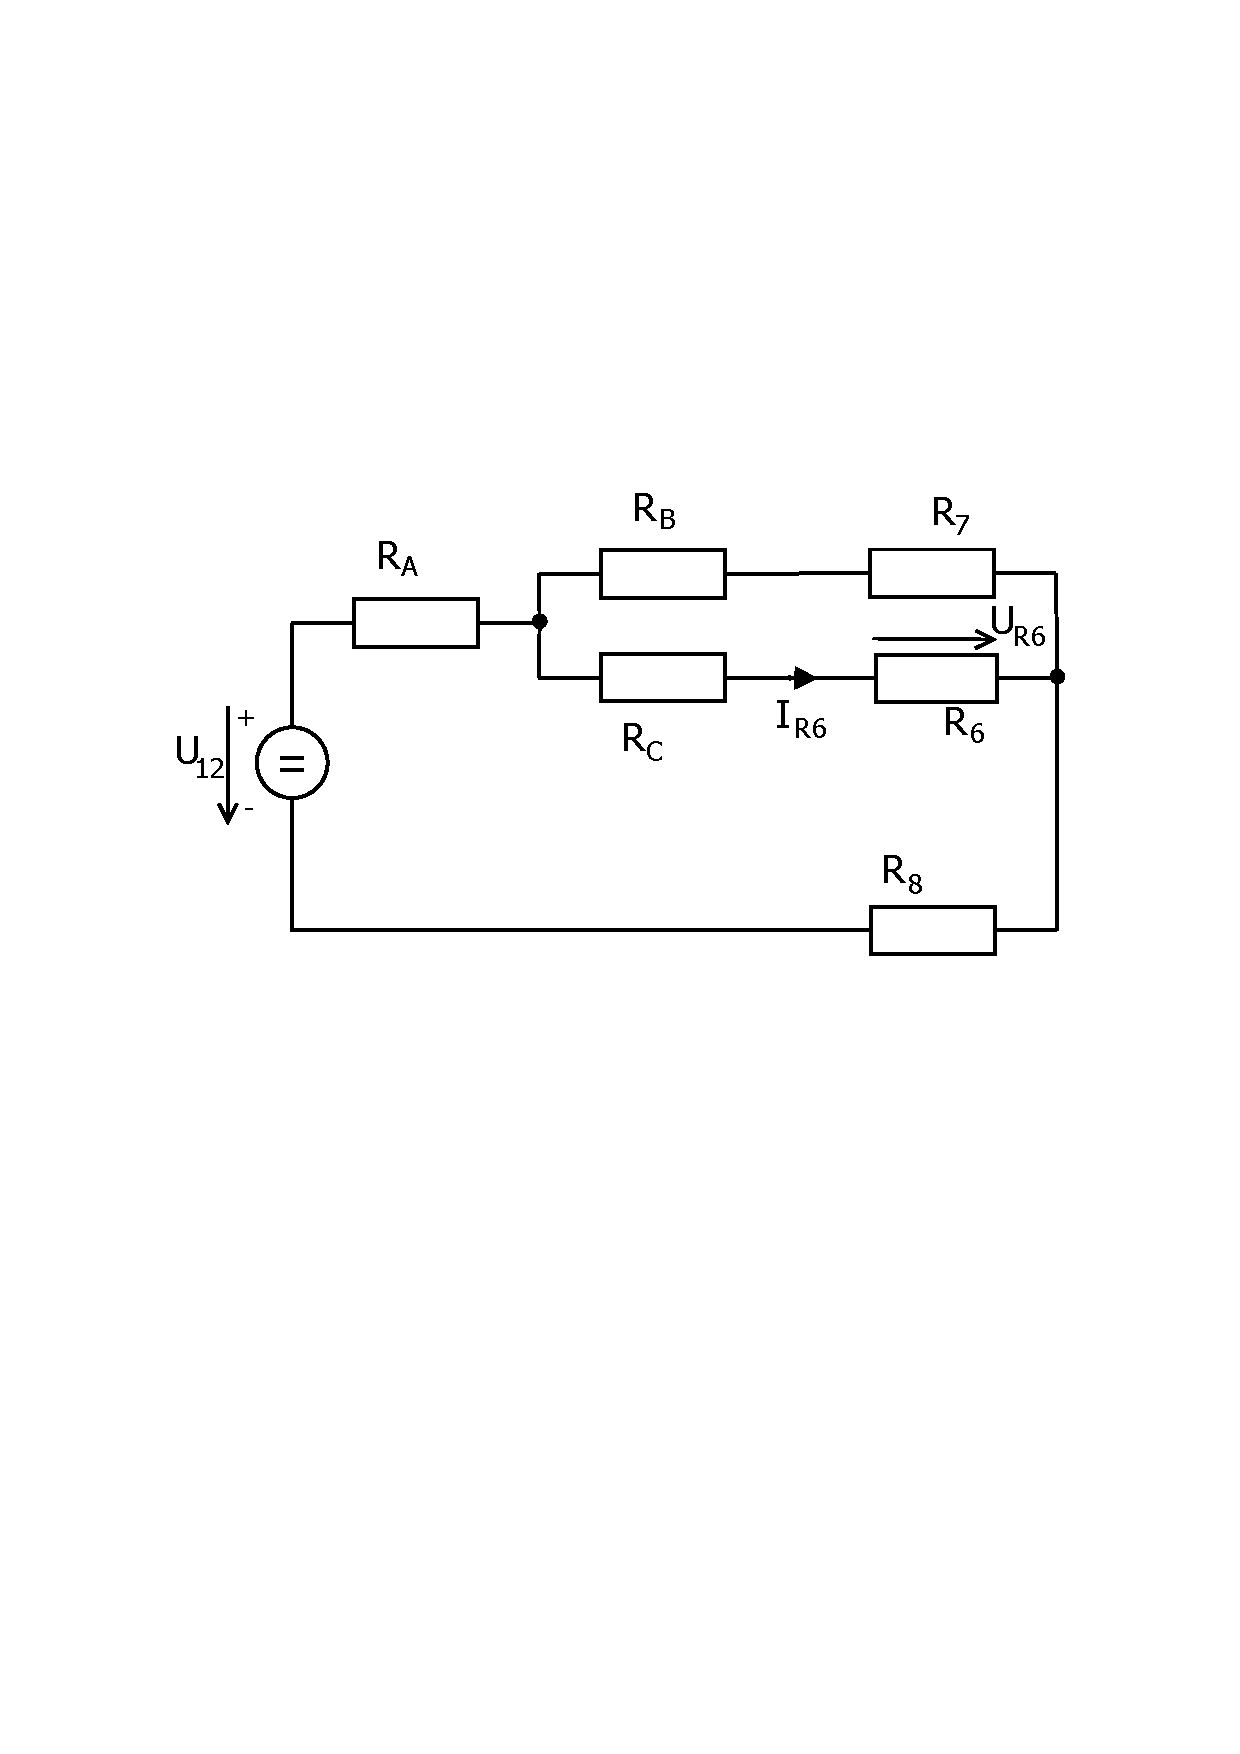
\includegraphics[width=0.6\linewidth]{obr/1_10}
		\caption*{Spočítáme si napětí a proud u $R_6$}
	\end{figure}
	\begin{gather*}
		I_{R_{C6}} = I_{R_6} = 0,0794 \text{A} \\
		U_{R_6} = {I_{R_6} R_6} = {0,0794 \cdot 830} = 65,902  \text{V} \\
	\end{gather*}
	
	\newpage